\documentclass{beamer}

% Theme selection
\usetheme{Madrid}
\usepackage{graphicx}

% Title slide information
\title{Classification of human breast leasons into \textbf{M}alignant and \textbf{B}enign in 3D ABUS}
\author{Ali Naderi Parizi, \\Dr. Mohsen Soryani}
\date{\today}

\begin{document}
	
\frame{\titlepage} % Title slide


\begin{frame}{Table of contents}
\tableofcontents
\end{frame}

\section{Problem statement}
\begin{frame}
	\frametitle{Problem statement}
	\begin{itemize}
		\item Having a 3D Volume of breast scanned using Ultrasound, we want to classify the detected leason.
		\item The leason mask which is the pixcelwise segmentation of real leason in the volume labeled by an expert radiologist is also present and we can eather include the mask in our training process or not. 
		\item There are two datasets available for the task: 
		\begin{enumerate}
			\item A private dataset collected for the segmentation task and might not be so helful in classification tasks. (due to class imbalance and high similarity between some cases in oposite classes.) 
			\item TDSC data set which is recently pulished for a global challenge consists of 100 samples (50 malignant - 50 benign) for training, 30 for validation and 70 for testcases. (Only training data is available)
		\end{enumerate}	
	\end{itemize}
\end{frame}

\begin{frame}
\begin{center}
		\begin{figure}
			\includegraphics[scale=0.8]{Sample.png}
			\centering
		\end{figure}
	\end{center}
\end{frame}

\section{3D-VGG Like networks}


\begin{frame}
	\frametitle{3D-VGG with input size of 64}
	\begin{center}
		\begin{figure}
			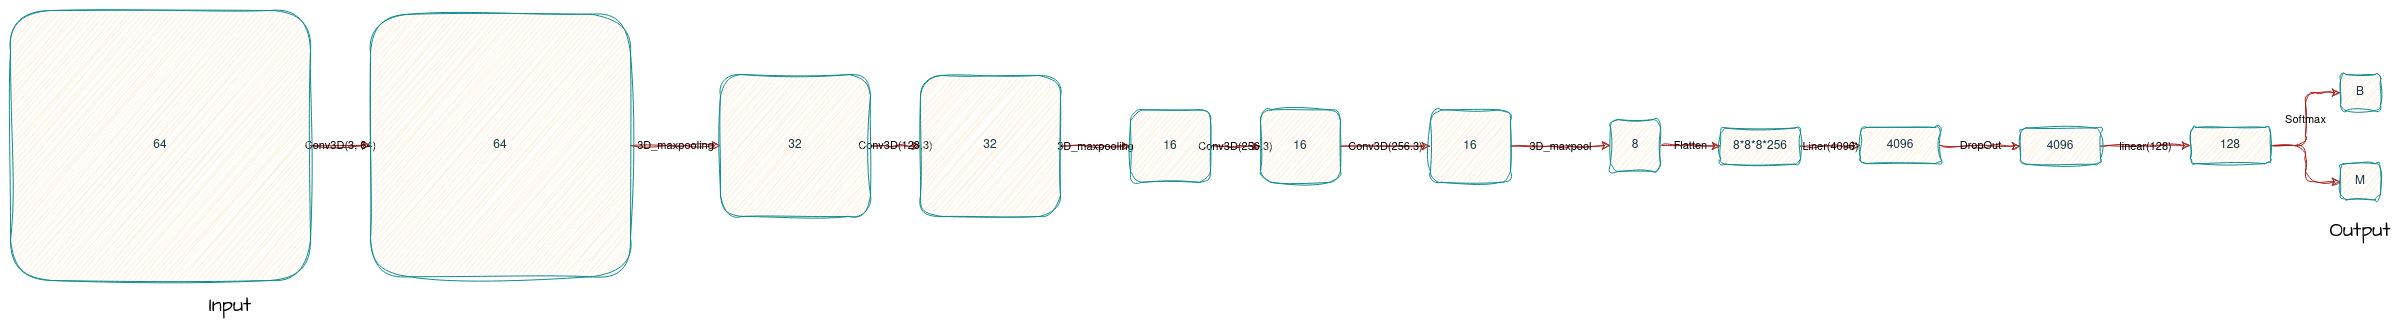
\includegraphics[scale=0.14]{3d-vgg.png}
			\centering
		\end{figure}
	\end{center}		
\end{frame}

\begin{frame}
	\frametitle{3D-VGG with input size of 64}
	\begin{block}{Network features}
		\begin{itemize}
			\item Convolutions: 3D convolutions.
			\item Loss function: Binary cross entropy loss
			\item Optimizer: Adam
		\end{itemize}
	\end{block}
	
	\begin{block}{Results}
		\begin{itemize}
			\item Private data set: Failur (52\% training accuracy)
			\item TDSC: Not tested yet.
		\end{itemize}
	\end{block}
\end{frame}

\begin{frame}
	\frametitle{Pretrained 3D-VGG with input size of 64}
	\begin{enumerate}
		\item Pretrain network using hande made shapes. (Triangle, Rectangle, circle, star, ...)
		\item Use non leason background for handcraft shapes.
	\end{enumerate}
\end{frame}

\section{2D VGG and LSTM}
\begin{frame}
	\frametitle{2D VGG and LSTM}
	\begin{center}
		\begin{figure}
			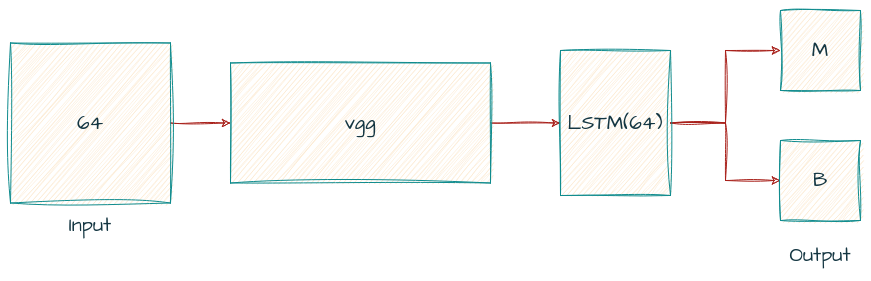
\includegraphics[scale=0.3]{vgg-lstm.png}
			\centering
		\end{figure}
	\end{center}
\end{frame}

\begin{frame}{2D VGG and LSTM}
	\begin{enumerate}
		\item Pretrain VGG.
		\item Pretrain VGG with handcrafted shapes.
		\item Pretrain VGG with handcraftd shapes and use non leason background.
	\end{enumerate}
\end{frame}


\section{Multitask Learning}
\begin{frame}{Multitask Learning}
	\begin{center}
		\begin{figure}
			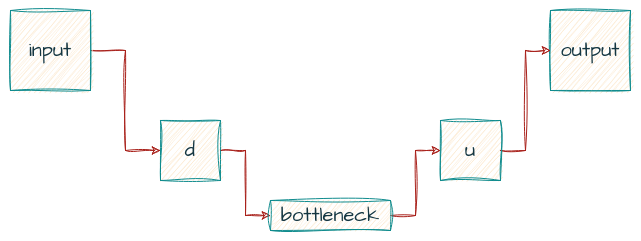
\includegraphics[scale=0.5]{unet.png}
			\centering
		\end{figure}
	\end{center}
\end{frame}

\section{Conclusion}
\begin{frame}
	\frametitle{Conclusion}
	\begin{itemize}
		\item The private dataset is not suitable for classification task and we  need a more balanced dataset.
		\item TDSC dataset is balanced but each silce is not related to its excesor and priors.
		\item Available model and papers should be tested on this dataset.
	\end{itemize}
\end{frame}

\end{document}